\documentclass[11pt,a4paper]{ctexart}

\usepackage[a4paper,margin=2.2cm]{geometry}
\usepackage{setspace}
\usepackage{graphicx}
\usepackage{booktabs}
\usepackage{array}
\usepackage{multirow}
\usepackage{amsmath,amssymb}
\usepackage{float}
\usepackage{caption}
\usepackage{subcaption}
\usepackage{xcolor}
\usepackage{hyperref}
\usepackage{titling}
\usepackage{enumitem}
\usepackage{tikz}
\usetikzlibrary{arrows.meta,positioning,shapes.geometric}

\definecolor{paperbg}{HTML}{F7F5F2}
\definecolor{ink}{HTML}{222222}
\definecolor{bluegray}{HTML}{A8B4C8}
\definecolor{steel}{HTML}{6C8EAD}
\definecolor{sand}{HTML}{D6A46A}
\definecolor{clay}{HTML}{D96C4F}
\definecolor{brick}{HTML}{8A1C1C}
\definecolor{sage}{HTML}{4B8466}
\definecolor{mist}{HTML}{EEF1F5}
\definecolor{linegray}{HTML}{D9DDE3}

\tikzset{
  paper diagram/.style={
    font=\small,
    >={Latex[length=2.2mm]},
    line cap=round,
    line join=round
  },
  stagebox/.style={
    draw=ink!90,
    rounded corners=4pt,
    line width=0.8pt,
    align=center,
    fill=paperbg,
    inner sep=6pt
  },
  bluebox/.style={
    stagebox,
    fill=bluegray!26,
    draw=ink!88
  },
  tealbox/.style={
    stagebox,
    fill=steel!22,
    draw=ink!88
  },
  warmbox/.style={
    stagebox,
    fill=sand!32,
    draw=ink!88
  },
  accentbox/.style={
    stagebox,
    fill=clay!24,
    draw=ink!88
  },
  tracebox/.style={
    stagebox,
    fill=mist,
    draw=ink!75
  },
  decisionbox/.style={
    draw=ink!90,
    diamond,
    aspect=2,
    line width=0.8pt,
    align=center,
    fill=clay!18,
    inner sep=1.8pt
  },
  flowarrow/.style={
    ->,
    draw=ink!88,
    line width=0.85pt
  },
  tracearrow/.style={
    ->,
    draw=ink!60,
    dashed,
    line width=0.75pt
  }
}

\hypersetup{
  colorlinks=true,
  linkcolor=blue!50!black,
  citecolor=blue!50!black,
  urlcolor=blue!60!black
}

\captionsetup{font=small,labelfont=bf}
\captionsetup[figure]{skip=6pt}
\captionsetup[table]{skip=4pt}
\setlength{\parskip}{0.45em}
\setlength{\parindent}{2em}
\linespread{1.2}
\emergencystretch=2em
\setlength{\droptitle}{-6.8em}
\pretitle{\begin{center}\LARGE\bfseries}
\posttitle{\par\end{center}\vspace{0em}}
\preauthor{\begin{center}\normalsize}
\postauthor{\par\end{center}\vspace{-0.4em}}
\predate{\begin{center}\small}
\postdate{\par\end{center}\vspace{-1.3em}}
\ctexset{
  section = {
    beforeskip = 1.5ex plus .2ex minus .1ex,
    afterskip = 0.9ex plus .1ex
  },
  subsection = {
    beforeskip = 1.1ex plus .1ex minus .1ex,
    afterskip = 0.6ex plus .1ex
  }
}
\renewenvironment{abstract}{
  \par\small
  \begin{center}\bfseries 摘要\end{center}
  \vspace{-0.6em}
  \noindent\ignorespaces
}{
  \par\vspace{0.2em}
}
\makeatletter
\setlength{\@fptop}{0pt}
\setlength{\@fpsep}{10pt}
\setlength{\@fpbot}{0pt plus 1fil}
\makeatother
\renewcommand{\topfraction}{0.92}
\renewcommand{\bottomfraction}{0.85}
\renewcommand{\textfraction}{0.07}
\renewcommand{\floatpagefraction}{0.8}

\title{\textbf{固定候选边界内的高可信语义路由}\\[0.35em]\large 结构化语义判别与受控协作复核}
\author{匿名稿}
\date{}

\begin{document}

\maketitle
\vspace{-0.8em}

\begin{abstract}
本文研究固定能力命名空间下的高可信语义路由，并聚焦一个更具体的问题：在候选集合已经冻结的前提下，协作复核究竟在什么条件下才能稳定带来净收益。与开放式文本生成不同，这一任务要求系统在候选集合内部完成主能力选择、相关能力恢复和执行落点解析，同时为每一次改判保留可复核证据和可审计路径。现有规则系统速度快但边界样本区分能力有限；一步式大模型裁决具备更强语义泛化能力，却往往缺乏稳定的候选内比较机制和可解释的改判边界。

本文提出一套固定候选边界内的受控路由框架。系统首先以 descriptor-only 召回定义 candidate-internal 搜索空间，再以结构化语义判别在候选集合内部生成候选级任务匹配、主能力判断和不确定性摘要；只有在低置信、高风险或多意图冲突样本上，系统才触发职责化协作复核，并通过共识排序与显式授权决定是否覆盖直接路由结果。整个推断过程以统一 trace contract 落盘，从而把“是否复核”和“是否允许改判”分解为可独立分析的问题。

我们在一个包含 \texttt{563} 条样本的冻结 benchmark 上进行评测。统一 \texttt{train/test} 主协议下，规则路由的 \texttt{test accuracy} 为 0.7876，结构化语义判别提升到 0.8761，加入默认协作复核后进一步达到 0.8850，\texttt{test acceptable accuracy} 为 0.9115。在更强的受控协作配置下，系统在同一 held-out \texttt{test} 集上达到 0.9292，并获得 \texttt{5 / 5 / 0} 的 \texttt{Changed / Fixed / Regressed} 结果；在扩展分布对齐子集上，同样的配置将结果从 0.8625 提升到 0.9250。

这些结果支持一个更窄但更稳的结论：固定候选边界内的主要性能台阶来自结构化语义判别，而协作复核只有在职责化证据与决策配置对齐时才稳定产生净收益。对于高可信语义路由，相比开放式多代理讨论，更有效的路径是候选内结构化判别加受控协作改判。
\end{abstract}

\noindent\textbf{关键词：}语义路由；智能体命名；多智能体协作；可审计决策；互联网基础资源

\section{引言}

随着大模型系统开始处理可调用能力、服务实例和受约束任务入口，互联网基础资源场景中的核心问题已经从“生成合理文本”转向“把请求稳定映射到正确的能力地址”。在这一设定下，用户输入往往同时携带主任务、次要诉求、场景线索和风险约束，系统不仅要在固定命名空间中做出主能力判断，还要恢复相关能力并落到可执行实例。这个问题表面上接近意图分类，实质上更接近受约束决策：输出空间固定，候选之间存在层级和语义耦合，错误必须能够定位到召回、候选内判断或执行落点的具体阶段。

现有方法通常落在两个极端。规则或轻量打分器在关键词命中充分时可以快速给出结果，但面对跨域重叠、父子节点冲突和多意图样本时容易失去区分能力。一步式大模型裁决具有更强的语义泛化能力，却往往缺乏稳定的候选内比较机制，也难以解释为什么改判某个 incumbent、为什么保留另一个竞争候选，或者为什么某次复核被触发而另一次没有。对于需要上线部署的互联网基础资源系统，这种缺少证据边界和责任归因的决策链会直接限制模型输出的可信使用。

本文关注的不是“多代理是否有用”这一宽泛问题，而是一个更可检验的问题：在固定候选边界内，协作复核究竟何时能够稳定带来净收益。我们的核心观点是，高可信语义路由的主要性能台阶来自候选内结构化语义判别；协作复核并不是默认有益的慢路径，而是一种只应在低置信、边界冲突或高风险条件下启动，并且必须接受显式改判授权的受控机制。换言之，本文要验证的是“结构化语义证据 + 受控协作改判”是否优于开放式多代理讨论。

围绕这一问题，我们提出一套固定候选边界内的受控路由框架。系统先通过 descriptor-only 召回定义搜索空间，再通过结构化语义判别产生候选级任务匹配、主能力判断和不确定性摘要；随后，系统只在特定条件下触发职责化协作复核，并通过角色专属证据视图、共识排序和改判授权决定是否覆盖直接路由结果。由此，“直接路由是否足够可靠”和“协作复核是否应该生效”被拆成两个可独立分析的问题。

我们在 \texttt{563} 条样本组成的冻结 benchmark 上评估这一框架。统一 \texttt{train/test} 主协议下，结构化语义判别将 \texttt{test accuracy} 从 0.7876 提升到 0.8761，默认协作复核进一步达到 0.8850；更强的受控协作配置在同一 held-out \texttt{test} 集上达到 0.9292，并获得 \texttt{5 / 5 / 0} 的 \texttt{Changed / Fixed / Regressed} 结果。在扩展分布对齐子集上，职责化协作同样把结果从 0.8625 提升到 0.9250。整体证据显示，协作收益不是普遍存在的，而是集中出现在职责化证据和决策配置对齐的边界样本上。

本文的贡献可以概括为三点：
\begin{itemize}[leftmargin=1.5em,itemsep=0.15em,topsep=0.25em]
\item 形式化固定候选边界内的高可信语义路由任务，将主能力选择、相关能力恢复和执行落点解析纳入统一问题定义，并明确 \texttt{candidate-internal} 约束。
\item 提出由结构化语义判别与受控协作复核组成的两阶段路由机制，把候选内语义判断、协作触发和改判授权拆分为可独立分析的决策环节。
\item 在 \texttt{563} 条样本的冻结 benchmark 上证明：主要性能台阶来自结构化语义判别，而协作复核只有在职责化证据与决策配置对齐时才稳定产生净收益。
\end{itemize}

\begin{figure}[tbp]
\centering
\resizebox{0.985\linewidth}{!}{%
\begin{tikzpicture}[paper diagram, node distance=0.8cm and 1.0cm]
\node[bluebox, text width=2.6cm] (input) {自然语言请求\\query + context};
\node[bluebox, right=of input, text width=2.7cm] (r) {候选召回\\descriptor-only recall\\$E_R(x)$};
\node[tealbox, right=of r, text width=2.8cm] (clean) {规则基线路由\\$s_{\mathrm{clean}}(c\mid x)$};
\node[warmbox, right=of clean, text width=3.1cm] (sem) {结构化语义判别\\$z_A(x),\,H(x),\,J(x)$};
\node[decisionbox, right=of sem, xshift=0.2cm] (gate) {触发协作?\\$g(x)$};
\node[accentbox, above right=0.55cm and 0.8cm of gate, text width=3.4cm] (review) {职责化协作复核\\role-specific evidence views};
\node[tracebox, below right=0.55cm and 0.8cm of gate, text width=3.5cm] (ctrl) {共识与授权\\$s_B(c)$ + authorize};
\node[tealbox, right=of ctrl, text width=2.8cm] (route) {最终语义路由\\$(\hat y,\hat R)$};
\node[bluebox, right=of route, text width=2.8cm] (endpoint) {执行落点解析\\$\hat a(\hat y)$};
\node[tracebox, below=1.35cm of sem, text width=13.7cm] (t) {统一 trace contract：candidate snapshot，decision packet，semantic handoff，role packets，override trace，endpoint trace};

\draw[flowarrow] (input) -- (r);
\draw[flowarrow] (r) -- (clean);
\draw[flowarrow] (clean) -- (sem);
\draw[flowarrow] (sem) -- (gate);
\draw[flowarrow] (gate) -- node[right, font=\footnotesize]{触发} (review);
\draw[flowarrow] (gate) -- node[right, font=\footnotesize]{直通} (ctrl);
\draw[flowarrow] (review.south) |- (ctrl.north);
\draw[flowarrow] (ctrl) -- (route);
\draw[flowarrow] (route) -- (endpoint);
\draw[tracearrow] (r) -- (t);
\draw[tracearrow] (clean) -- (t);
\draw[tracearrow] (sem) -- (t);
\draw[tracearrow] (review) -- (t);
\draw[tracearrow] (ctrl) -- (t);
\draw[tracearrow] (endpoint) -- (t);
\end{tikzpicture}
}
\caption{系统总体架构。候选召回首先定义 candidate-internal 搜索边界；直接路由路径在该边界内产生候选级结构化判断；协作复核只在升级条件满足时触发，并通过显式授权控制 override 是否生效。}
\label{fig:architecture}
\end{figure}

\section{相关工作与问题定位}

与本文最接近的一类工作是 LLM routing。RouteLLM、MixLLM 等方法研究的是按查询在多个模型之间进行分配，并围绕质量、成本和延迟学习路由策略\cite{routellm,mixllm}。这类工作关心的是模型级选择，而本文处理的是能力级语义路由：系统必须在单一能力命名空间内选出正确的 \texttt{routing\_fqdn}，同时恢复 related 能力并维持改判边界的可审计性。因此，两者虽然都属于 routing，但决策对象、错误来源和评价目标并不相同。模型路由优化的是质量--成本权衡；本文优化的是固定候选边界内的主能力判断、related 恢复和协作改判质量。

第二类相关工作来自大模型推理增强。Chain-of-Thought、Self-Consistency 和 Tree of Thoughts 证明了多路径推理、采样一致性和显式搜索能够提升复杂推理表现\cite{cot,selfconsistency,tot}。这些方法的重要启发在于：当任务存在多个竞争解释时，单一步骤推断往往不足，需要把中间判断显式展开。然而，上述工作大多面向开放输出空间，较少要求系统在冻结候选集内完成主标签、相关标签和风险边界的联合决策。本文借鉴了显式保留中间语义判断的思想，并将其进一步落实到固定候选边界内的受约束决策。

第三类相关工作来自多智能体讨论与反馈式协作\cite{debate}. 这一路线的核心假设是，多视角复核可以缓解单模型的局部盲点。与此同时，近期研究也表明，多智能体讨论的收益并不稳定，控制协议和任务结构往往比“代理数量”更关键\cite{bounds}。这一结论与本文的观察高度一致。本文关注的是如何让职责化证据进入最终决策链路，并将“复核是否有信息增益”和“改判是否被允许”拆成两个可独立分析的问题。

此外，Constitutional AI 等反馈约束方法说明，规则和反馈信号能够有效塑造模型的行为边界\cite{cai}。本文沿着这一思路，将治理约束、角色责任和 override 授权显式写入受限决策流程，使规则边界与语义判断在同一协议下协同工作。

据此，本文的问题定位更接近受控 routing，而不是通用的讨论式推理。它继承了 routing 文献关于“按查询做选择”的基本视角，吸收了显式中间判断和多角色复核的启发，但把研究重点落在固定命名空间、candidate-internal 决策以及可回放 trace 上。本文因此既不同于以质量--成本权衡为目标的模型路由，也不同于输出空间开放、难以界定改判边界的通用多代理讨论。

\section{方法}

\subsection{问题表述与方法概览}

本文的方法围绕一个中心分解展开：先在冻结候选集合内部建立可靠的结构化语义判断，再只在直接路由证据不足时触发受控协作复核。换言之，本文并不把协作复核视为默认有益的通用慢路径，而把它视为一种建立在高质量语义交接之上的条件化改判机制。候选召回、规则路由和执行落点解析是支撑这一中心分解的三个边界模块：召回定义搜索边界，规则路由提供可解释基线，执行落点解析负责把已经确定的能力地址映射到具体实例。

本文区分两类核心语义对象。第一类是能力地址 \texttt{routing\_fqdn}，用于表示请求应被哪一类能力处理；第二类是实例地址 \texttt{agent\_fqdn}，用于表示在该能力下由哪个具体实例执行。能力地址要求语义稳定，实例地址允许随运行环境和服务状态动态变化。通过显式区分这两个层级，系统可以把“语义路由是否正确”和“执行落点是否合适”分开建模。

设能力命名空间为 $\mathcal{N}=\{c_1,\ldots,c_M\}$，输入请求表示为 $x=(q,m)$，其中 $q$ 为自然语言查询，$m$ 为可选上下文元信息，如领域、场景和风险线索。系统输出记为
\begin{equation}
F(x)=\bigl(\hat y(x), \hat R(x), \hat a(x)\bigr),
\end{equation}
其中 $\hat y(x)\in\mathcal{N}$ 表示主能力地址，$\hat R(x)\subseteq\mathcal{N}\setminus\{\hat y(x)\}$ 表示相关能力集合，$\hat a(x)\in A(\hat y(x))$ 表示执行实例。主评测集中在 $\hat y(x)$ 与 $\hat R(x)$ 的正确性，执行落点解析作为下游步骤独立建模。

方法设计遵循一个关键约束：所有下游决策都必须发生在候选召回返回的集合内部。记候选召回模块返回的有序集合为 $C_R(x)=\{c_1,\dots,c_K\}\subseteq\mathcal{N}$，则本文要求
\begin{equation}
\hat y(x)\in C_R(x), \qquad \hat R(x)\subseteq C_R(x)\setminus\{\hat y(x)\}.
\end{equation}
这一 \texttt{candidate-internal} 约束使错误能够被清晰拆解为两类：若真值不在 $C_R(x)$ 中，则属于召回错误；若真值已被召回但最终选择错误，则属于候选内裁决错误。本文所有方法设计和实验分析都建立在这一区分之上，因为本文要验证的正是候选内结构化判别与受控改判能否带来增益。

在推断层面，系统先由召回模块构造候选证据包，再由直接路由路径产生初始主能力与相关能力预测，随后由决策配置决定是否触发协作复核，最后在必要时将能力地址解析到实例地址。形式上，本文将这一流程写为
\begin{equation}
C_R(x)\rightarrow z_A(x)\rightarrow g(x)\rightarrow z_B(x)\rightarrow \hat a(x),
\end{equation}
其中 $z_A(x)$ 表示直接路由输出，$g(x)\in\{0,1\}$ 表示是否升级到协作复核，$z_B(x)$ 表示协作复核后的最终路由结果。这个分解把本文的核心命题写成三个可分解问题：候选集合是否覆盖真值、主能力是否在候选内被正确选出，以及协作复核是否在保留审计边界的前提下带来净修正。

\subsection{候选召回}

候选召回模块的目标是在能力命名空间中组织高覆盖、低泄漏的候选集合。本文采用 descriptor-only 的 clean recall 方案，仅使用节点描述、别名、层级信息与元数据标签完成词法和元数据融合召回，以避免把下游决策信号提前泄漏到召回阶段。

对每个候选 $c\in\mathcal{N}$，召回模块计算
\begin{equation}
S_R(c\mid x)=\lambda_1 \phi_{\text{alias}}(q,c)+\lambda_2 \phi_{\text{desc}}(q,c)+\lambda_3 \phi_{\text{hier}}(q,c)+\lambda_4 \phi_{\text{meta}}(m,c)-\lambda_5 \phi_{\text{over}}(c),
\end{equation}
其中 $\phi_{\text{alias}}$ 表示查询与别名的匹配强度，$\phi_{\text{desc}}$ 表示查询与节点描述的匹配强度，$\phi_{\text{hier}}$ 表示层级一致性信号，$\phi_{\text{meta}}$ 表示场景元信息与节点标签的匹配，$\phi_{\text{over}}$ 表示过度具体或层级失衡带来的惩罚项。系统按 $S_R(c\mid x)$ 排序并截取 top-$K$ 作为候选集合 $C_R(x)$。

召回模块的输出是一份可供后续模块复用的候选证据包
\begin{equation}
E_R(x)=\{(c, s_R(c), d_c, a_c, h_c, m_c)\mid c\in C_R(x)\},
\end{equation}
其中 $d_c$、$a_c$、$h_c$ 和 $m_c$ 分别表示描述、别名、层级位置与元数据快照。由于后续所有模块都只能访问 $E_R(x)$ 中的候选，召回模块实际定义了整个系统的搜索边界。本文在主文中不把召回写成主要创新点；它的作用是为后续候选内判别提供高覆盖、低泄漏的搜索空间。

\subsection{规则路由}

规则路由（Rule-based Router）是系统的确定性直接路由器。它在 $E_R(x)$ 上计算候选级主任务分数，并为后续模块提供统一的候选内基线。与“只看一次文本相似度”的轻量规则不同，该模块显式融合召回分数强度、主任务命中、上下文匹配、层级粒度、证据多样性和节点类型适配，同时施加结构性惩罚。

对每个候选 $c\in C_R(x)$，规则路由计算主路由分数
\begin{equation}
\label{eq:clean-primary}
\begin{aligned}
s_{\mathrm{clean}}(c\mid x)=\;&
\omega_r \tilde s_R(c)
+ \omega_p \phi_{\mathrm{pri}}(c)
+ \omega_c \phi_{\mathrm{ctx}}(c)
+ \omega_h \phi_{\mathrm{hier}}(c)\\
&+ \omega_s \phi_{\mathrm{spec}}(c)
+ \omega_d \phi_{\mathrm{div}}(c)
+ \omega_n \phi_{\mathrm{node}}(c)
- \Pi_{\mathrm{struct}}(c),
\end{aligned}
\end{equation}
其中 $\tilde s_R(c)$ 是召回分数归一化结果，$\phi_{\mathrm{pri}}$ 表示主任务命中强度，$\phi_{\mathrm{ctx}}$ 表示上下文匹配，$\phi_{\mathrm{hier}}$ 表示层级支持，$\phi_{\mathrm{spec}}$ 表示粒度适配，$\phi_{\mathrm{div}}$ 表示证据多样性，$\phi_{\mathrm{node}}$ 表示节点类型适配，$\Pi_{\mathrm{struct}}(c)$ 表示结构性惩罚项。主能力基线预测写为
\begin{equation}
\hat y_{\mathrm{clean}}(x)=\arg\max_{c\in C_R(x)} s_{\mathrm{clean}}(c\mid x).
\end{equation}

给定 $\hat y_{\mathrm{clean}}$ 之后，系统再在非链重复候选中恢复 related 集合。该步骤使用 secondary 支持、补充子句线索、上下文匹配和与主能力的关系加成进行打分，并通过父子链去重与阈值约束抑制冗余 related。其精确权重与阈值配置见 Appendix~\ref{appendix:prompt-contracts}。这一模块的作用有两个：一是提供可解释的强基线，二是为结构化语义判别提供稳定的融合底座。

\subsection{结构化语义判别}

结构化语义判别（Structured Semantic Routing）是本文的主增益来源。它在规则路由之上引入受约束的大模型判断，但并不直接输出最终标签，而是读取 top-$K$ 候选 decision packet，并返回一组受约束的结构化字段：主能力候选、related 候选、候选级 \emph{task fit / primary fit / related fit}、粒度判断、风险失配标记，以及用于下游协作复核的语义交接信息。其输出写为
\begin{equation}
z_A(x)=\bigl(\hat y_A,\hat R_A,s_A,H(x),J(x)\bigr),
\end{equation}
其中 $H(x)$ 表示语义交接字段，编码场景摘要、主任务摘要、次任务摘要、不确定性摘要、混淆点和改判敏感性；$J(x)$ 表示候选级结构化判断表。

随后，系统将规则分数与结构化语义判断进行候选内融合。对每个候选 $c$，主路由融合分数定义为
\begin{equation}
\label{eq:semantic-primary}
s_A(c\mid x)=
\alpha_1 \widetilde s_{\mathrm{clean}}(c)
+ \alpha_2 \widetilde s_R(c)
+ \alpha_3 f_{\mathrm{task}}(c)
+ \alpha_4 f_{\mathrm{pri}}(c)
+ b_{\mathrm{sel}}(c)
+ \delta_{\mathrm{spec}}(c)
- \delta_{\mathrm{risk}}(c),
\end{equation}
其中 $\widetilde s_{\mathrm{clean}}$ 是规则主路由分数归一化，$f_{\mathrm{task}}$ 和 $f_{\mathrm{pri}}$ 分别对应 LLM 输出的 \emph{task fit} 与 \emph{primary fit}，$b_{\mathrm{sel}}$ 奖励被 LLM 显式选为 primary 的候选，$\delta_{\mathrm{spec}}$ 表示粒度判断修正，$\delta_{\mathrm{risk}}$ 表示风险失配惩罚。related 恢复采用与式(\ref{eq:semantic-primary})同构的融合模板，并结合 parent-child guard、generic trigger alias guard 和 explicit cue guard 抑制过细粒度误选。

直接路由置信度由 route probability、top-1/top-2 margin、LLM 证据支持度和与规则路由的一致性共同决定。当置信度过低、margin 过小、LLM 主动请求升级、高风险条件未充分满足，或多意图样本未能恢复 related 时，样本被送入协作复核。对本文而言，这一步的关键不只是把正确标签选出来，更是形成一份足够高质量的语义交接，使后续协作复核在边界样本上真正有信息可用。融合细节、置信校准和 related 打分模板见 Appendix~\ref{appendix:prompt-contracts}。

\subsection{职责化协作复核}

职责化协作复核（Collaborative Review）负责处理低置信、margin 过小、高风险和多意图冲突样本。它在候选集合内部执行职责约束下的复核，而不重新打开开放式输出空间。本文把这一模块写成受控改判器，而不是通用多代理讨论器：角色的作用是补充不同维度的证据，而不是自由扩展输出空间。本文采用四类职责角色：\texttt{DomainExpert} 负责任务匹配，\texttt{GovernanceRisk} 负责治理与风险审查，\texttt{HierarchyResolver} 负责层级与粒度冲突，\texttt{UserPreference} 负责主次意图拆分与偏好线索。

对每个角色 $r\in\mathcal R$，系统从共享证据包中构造角色专属视图
\begin{equation}
P_r(x)=\Pi_r\bigl(E_R(x),z_A(x),H(x)\bigr).
\end{equation}
例如，\texttt{DomainExpert} 主要访问任务匹配与正证据卡，\texttt{GovernanceRisk} 主要访问风险边界与负证据卡，\texttt{HierarchyResolver} 主要访问 parent-child 与 granularity 线索，\texttt{UserPreference} 主要访问 secondary anchors 与 primary/secondary 分离线索。角色 $r$ 的输出定义为
\begin{equation}
o_r(x)=\bigl(\hat y_r,\hat R_r,\rho_r,\kappa_r,\sigma_r\bigr),
\end{equation}
其中 $\hat y_r$ 和 $\hat R_r$ 是角色提案，$\rho_r$ 是角色置信度，$\kappa_r\in\{\texttt{support\_stage\_a},\texttt{propose\_override}\}$ 表示是否支持改判，$\sigma_r$ 是职责维度上的 role signal（support / block / neutral）。

控制器首先在 round-1 汇总角色投票，得到候选级复核分数
\begin{equation}
\label{eq:round1-consensus}
s_B^{(1)}(c\mid x)=
0.40\,\mathrm{vote\_ratio}(c)
+0.25\,\overline{\rho}(c)
+0.15\,s_A(c)
+0.10\,\mathrm{explicit}(c)
+0.10\,\mathrm{rel\_vote}(c)
+\mathrm{signal}(c),
\end{equation}
其中 $\mathrm{vote\_ratio}(c)$ 表示把 $c$ 作为 primary 的角色比例，$\overline{\rho}(c)$ 表示这些角色的平均置信度，$\mathrm{explicit}(c)$ 表示候选显式证据强度，$\mathrm{rel\_vote}(c)$ 表示把 $c$ 挂为 related 的比例，$\mathrm{signal}(c)$ 表示异质角色 support/block 信号的带符号加权和。若 round-1 的 top-1/top-2 间隔过小，或 top-1 相对直接路由 incumbent 构成敏感 override（高风险、跨 L1、层级改判），系统触发 round-2，只在 winner 与关键 challenger 或 incumbent 之间重判。最终共识分数在 round-1、round-2 和直接路由证据之间插值融合，精确配比见 Appendix~\ref{appendix:prompt-contracts}。

改判生效还需经过显式授权检查。若 winner 相对直接路由 incumbent 构成 override，则系统要求同时满足：足够的 override 票数、足够的共识分数增益、足够强的显式主任务证据；对于高风险、跨 L1 或层级改判，还额外要求 round-2 共识、主任务显式命中增强，以及相应职责角色的责任确认。由此，协作复核被实现为“角色提案 + 共识排序 + 授权检查”的三段式控制器。这个设计的目的不是增加额外推理步数，而是把“哪些证据允许改判”明确写入决策链。

\subsection{协作触发与改判授权}

协作复核不会对所有样本无差别触发，其入口由决策配置控制。系统首先基于直接路由输出构造升级分数
\begin{equation}
G(x)=\eta_1\bigl(1-s_A\bigr)+\eta_2 \,\mathrm{margin}^{-1}(x)+\eta_3 \,\rho(x)+\eta_4 \,\mu(x)+\eta_5 \,\kappa(x),
\end{equation}
其中 $s_A$ 为直接路由置信度，$\mathrm{margin}(x)$ 表示 top-1/top-2 间隔，$\rho(x)$ 表示风险强度，$\mu(x)$ 表示多意图迹象，$\kappa(x)$ 表示层级冲突或跨域竞争信号。升级决策定义为
\begin{equation}
g(x)=\mathbb{I}\{G(x)>\tau_g\},
\end{equation}
其中 $\tau_g$ 由具体决策配置决定。本文比较的几种配置本质上对应不同的复核触发阈值与改判门槛。若样本未升级，则系统保留直接路由结果；若样本升级，则只在复核分数超过最终改判门槛时接受协作修正。这个分离式设计将“是否值得复核”与“是否允许最终改判”解耦，也使本文能够在实验中分别分析语义证据质量和决策配置的贡献。详细阈值和判定模板见 Appendix~\ref{appendix:prompt-contracts}。

\begin{figure}[tbp]
\centering
\resizebox{0.94\linewidth}{!}{%
\begin{tikzpicture}[paper diagram, node distance=0.75cm and 0.7cm]
\node[tracebox, text width=4.0cm] (shared) {共享证据包\\$E_R(x),\,z_A(x),\,H(x)$};
\node[bluebox, below left=0.95cm and 3.75cm of shared, text width=2.45cm] (domain) {Domain\\Expert\\task match\\positive evidence};
\node[accentbox, below=0.95cm of shared, text width=2.45cm] (gov) {Governance\\Risk\\risk boundary\\negative evidence};
\node[warmbox, right=of gov, text width=2.45cm] (hier) {Hierarchy\\Resolver\\parent-child\\granularity};
\node[tealbox, right=of hier, text width=2.45cm] (pref) {User\\Preference\\primary-secondary\\intent split};
\node[tracebox, below=1.25cm of gov, text width=4.2cm] (vote) {round-1 聚合\\$\hat y_r,\hat R_r,\rho_r,\kappa_r,\sigma_r$};
\node[decisionbox, right=1.1cm of vote] (round2) {需要\\round-2?};
\node[warmbox, above right=0.55cm and 0.9cm of round2, text width=3.15cm] (r2) {winner vs incumbent/challenger\\targeted re-check};
\node[accentbox, below right=0.55cm and 0.9cm of round2, text width=3.2cm] (auth) {授权检查\\votes + score delta + role responsibility};
\node[tealbox, below=1.1cm of auth, text width=2.7cm] (final) {最终 $(\hat y,\hat R)$};

\draw[flowarrow] (shared) -- (domain);
\draw[flowarrow] (shared) -- (gov);
\draw[flowarrow] (shared) -- (hier);
\draw[flowarrow] (shared) -- (pref);
\draw[flowarrow] (domain.south) |- (vote.west);
\draw[flowarrow] (gov) -- (vote);
\draw[flowarrow] (hier.south) |- (vote.east);
\draw[flowarrow] (pref.south) |- (vote.east);
\draw[flowarrow] (vote) -- (round2);
\draw[flowarrow] (round2) -- node[right, font=\footnotesize]{是} (r2);
\draw[flowarrow] (round2) -- node[right, font=\footnotesize]{否} (auth);
\draw[flowarrow] (r2.south) |- (auth.north);
\draw[flowarrow] (auth) -- (final);
\end{tikzpicture}
}
\caption{职责化协作复核流程。角色看到的是职责投影后的证据视图。控制器先聚合 round-1 提案，再按需要触发 winner 与 incumbent/challenger 的 round-2 复核，并在最终 override 前执行授权检查。}
\label{fig:flow}
\end{figure}

\subsection{过程记录与可审计性}

本文将“可信”界定为工程上可审计、可回放、可归因的结构化行为链。对每个样本，系统记录
\begin{equation}
T(x)=\bigl(E_R(x), z_{\mathrm{clean}}(x), z_A(x), g(x), \{o_r(x)\}_{r\in\mathcal{R}}, z_B(x), \hat a(x)\bigr),
\end{equation}
其中包含候选快照、直接路由输出、升级信号、角色提案、角色可见视图、最终改判来源和执行落点。这样的统一过程记录结构使系统不仅输出最终结果，还能够明确说明结果形成路径、错误来源归属以及某次协作复核改判的具体证据驱动。

这种 trace 机制同时服务于方法评价与工程审计。从研究角度看，它支持将错误分析回溯到具体阶段和具体样本；从系统角度看，它为后续加入 hash-chain、篡改检测和跨系统对账等机制提供了统一数据结构基础。

\subsection{执行落点解析}

在能力地址裁决之后，系统还需要将 \texttt{routing\_fqdn} 落到具体执行实例。执行落点解析模块负责在实例集合 $A(\hat y)$ 中完成这一步。该模块坚持四项约束：只接受 exact \texttt{routing\_fqdn} match 的实例；不在执行层改写能力地址；不在执行选择中再次引入 LLM；对离线、缺失 endpoint 或 schema 不兼容实例进行硬过滤。在此基础上，系统使用由语义匹配、schema 兼容、服务标签、健康度和公平曝光组成的可解释评分函数，对候选实例排序。其评分公式写为
\begin{equation}
\text{final}(a)=\text{base}(a)\cdot \text{health}(a)\cdot \text{fair}_{\text{agent}}(a)\cdot \text{fair}_{\text{provider}}(a),
\end{equation}
其中
\begin{equation}
\text{base}(a)=0.55\,S_{\text{match}}(a)+0.25\,S_{\text{schema}}(a)+0.20\,S_{\text{tag}}(a).
\end{equation}
这一步不再改变语义路由结果，只在给定能力地址的条件下选择可执行实例。因而，它与上游语义裁决模块在功能上保持解耦：前者决定“做什么”，后者决定“由谁来做”。

\section{实验}

\subsection{数据资产}

围绕智能体命名与语义路由任务，本文整理得到总计 \texttt{563} 条样本的数据资产，并冻结划分为统一的 \texttt{train=450} 和 \texttt{test=113}。主文所有核心结论都建立在这一 held-out benchmark 之上，而不是建立在若干彼此并列的小规模测试集上。

数据标签围绕能力命名空间展开，主标签为 \texttt{ground\_truth\_fqdn}，同时支持 \texttt{acceptable\_fqdns} 与 \texttt{relevant\_fqdns}，以覆盖层级合理回落和相关能力恢复这两类更贴近真实路由系统的现象。与单纯的分类任务不同，这一标注设计允许系统区分“主能力是否选对”和“辅助能力是否恢复充分”。

除统一主协议外，本文还在冻结 benchmark 上定义了一组后验诊断视角，用于分析协作复核在何种类型样本上产生修正，例如常规揭盲样本、困难边界样本、fresh 样本和扩展分布样本。它们只服务于结果解释、失败模式分析和协作消融，而不作为独立数据集组成主叙事。

\begin{figure}[tbp]
\centering
\resizebox{0.88\linewidth}{!}{%
\begin{tikzpicture}[paper diagram, node distance=0.9cm and 1.1cm]
\node[tracebox, text width=3.5cm] (pool) {冻结 benchmark\\\textbf{563 examples}};
\node[bluebox, below left=1.05cm and 1.45cm of pool, text width=2.9cm] (train) {Train split\\\textbf{450}};
\node[accentbox, below right=1.05cm and 1.45cm of pool, text width=2.9cm] (test) {Held-out test\\\textbf{113}};
\node[tealbox, below=1.05cm of train, text width=4.8cm] (slices) {训练阶段用途\\配置开发，阈值选择，误差分析，消融比较};
\node[warmbox, below=1.05cm of test, text width=4.8cm] (eval) {测试阶段用途\\统一主结果，后验诊断，协作消融报告};

\draw[flowarrow] (pool) -- (train);
\draw[flowarrow] (pool) -- (test);
\draw[flowarrow] (train) -- (slices);
\draw[flowarrow] (test) -- (eval);
\end{tikzpicture}
}
\caption{数据与评测协议。本文首先在 \texttt{563} 条样本上冻结统一 \texttt{train/test} 主协议；所有主表结论基于同一 held-out benchmark，后验诊断和协作消融则用于解释修正来源和边界样本收益。}
\label{fig:protocol}
\end{figure}

\subsection{评测协议与指标}

主评测协议采用冻结的统一 \texttt{train/test} 划分，并以 \texttt{Train Acc}、\texttt{Test Acc}、\texttt{Test Acceptable} 和 \texttt{C/F/R} 等指标报告系统表现。所有 prompt、权重和决策配置均在训练划分上开发，held-out \texttt{test} 集仅用于最终结果报告。在这一主协议之外，本文还开展两类后验分析：其一是诊断性子集分析，用于观察修正收益主要出现在哪些类型的样本上；其二是扩展分布上的协作消融，用于分析角色异质性与决策配置的配合关系。由此，主统计结果、诊断分析和机制消融共同构成本文的证据体系。

系统主要报告四类指标。第一，主标签准确率衡量主能力是否正确。第二，可接受主标签准确率允许命中预定义的等价标签。第三，相关能力召回率和精确率用于评估相关能力恢复的完整性与准确性。第四，系统还记录协作复核触发率、修正计数和错误桶分布，用于分析协作复核是否真正带来修正，以及错误主要集中在召回、主标签判断还是 related 恢复层面。

表中的 \texttt{C/F/R} 是诊断指标，分别表示 \texttt{Changed}、\texttt{Fixed} 和 \texttt{Regressed}。其中，\texttt{Changed} 表示协作复核路径相对于对应直接路由路径改写了多少个测试样本的主预测；\texttt{Fixed} 表示这些改写中有多少个把原本错误的样本修正为正确；\texttt{Regressed} 表示其中有多少个把原本正确的样本改坏。它用于刻画协作复核改判的净收益和风险边界，是对准确率的补充解释，不能替代准确率主指标。

\section{实验结果}

\subsection{统一 train/test 主结果}

本文最核心的结果来自统一 \texttt{train/test} 主协议，如表~\ref{tab:pooled-main} 所示。

\begin{table}[H]
\centering
\caption{统一 \texttt{train/test} 主协议下的系统结果。\texttt{C/F/R} 分别表示 Changed、Fixed、Regressed。}
\label{tab:pooled-main}
\begin{tabular}{lcccc}
\toprule
系统 & Train Acc & Test Acc & Test Acceptable & Test C/F/R \\
\midrule
规则路由 & 0.8156 & 0.7876 & 0.8142 & -- \\
规则路由 + 协作复核 & 0.8244 & 0.8053 & 0.8319 & 2 / 2 / 0 \\
结构化语义判别 & 0.8756 & 0.8761 & 0.9027 & -- \\
结构化语义判别 + 协作复核 & 0.8844 & 0.8850 & 0.9115 & 1 / 1 / 0 \\
\bottomrule
\end{tabular}
\end{table}

主表显示，两级直接路由已经能够建立清晰的性能台阶。与规则路由相比，结构化语义判别将 \texttt{test accuracy} 从 0.7876 提升到 0.8761，将 \texttt{test acceptable accuracy} 从 0.8142 提升到 0.9027；在此基础上加入协作复核，系统进一步达到 0.8850 和 0.9115，并保持零回归。该结果说明，主要增益首先来自候选内语义判别质量的提升，协作复核则在边界样本上继续提供净修正。

\begin{figure}[tbp]
\centering

\includegraphics[width=0.92\linewidth]{figures/01_pooled_test_waterfall.pdf}
\caption{统一 \texttt{train/test} 主协议下的系统增益瀑布图。主要性能跨越来自规则路由到结构化语义判别的跃迁，而角色协作复核主要承担后段修正。}
\label{fig:waterfall}
\end{figure}

\subsection{何时协作复核有效：决策配置对比}

在统一 \texttt{train/test} 主协议下，系统进一步比较三种协作决策配置，结果如表~\ref{tab:gate} 所示。

\begin{table}[H]
\centering
\caption{统一 \texttt{train/test} 主协议下的协作决策配置结果。}
\label{tab:gate}
\begin{tabular}{lcccc}
\toprule
配置 & Train Acc & Test Acc & Test C/F/R & 相对默认配置提升 \\
\midrule
\texttt{default} & 0.8800 & 0.8850 & -- & 0.0000 \\
\texttt{selective} & 0.8911 & 0.8938 & 1 / 1 / 0 & +0.0088 \\
\texttt{expanded} & 0.8978 & 0.9292 & 5 / 5 / 0 & +0.0442 \\
\bottomrule
\end{tabular}
\end{table}

\texttt{expanded} 配置在统一 \texttt{test} 集上达到 0.9292，相对 \texttt{default} 提升 0.0442，并实现 \texttt{5 / 5 / 0} 的诊断结果，即 5 次改写全部转化为有效修正且没有引入回归；\texttt{selective} 也保持 \texttt{1 / 1 / 0}。进一步检查样本级结果可以看到，\texttt{expanded} 的新增修正主要集中在扩展分布样本上。这说明配置收益不是平均发生在所有样本上，而是主要体现在高价值边界样本中。

\begin{figure}[tbp]
\centering
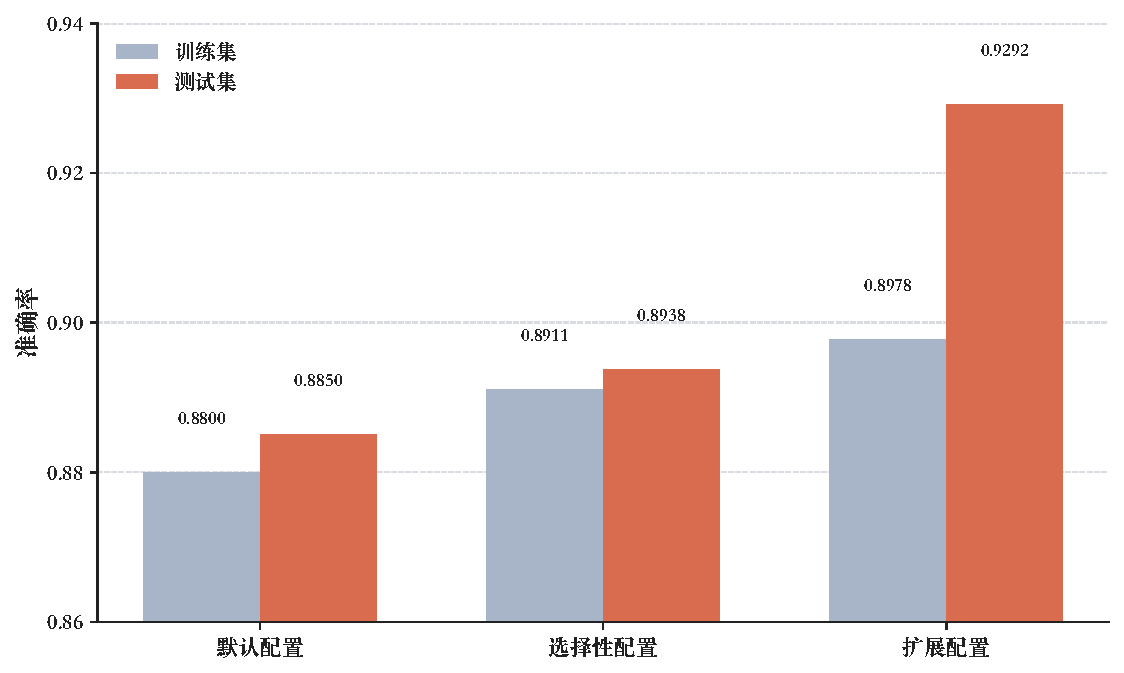
\includegraphics[width=0.80\linewidth]{figures/02_pooled_gate_selection.pdf}
\caption{统一 \texttt{train/test} 主协议上的协作决策配置结果。\texttt{expanded} 在训练划分和测试划分中均表现最优。}
\label{fig:gate-selection}
\end{figure}

\subsection{何种协作形式有效：协作复核消融}

在扩展分布对齐子集上，结构化语义判别的 \texttt{test accuracy} 为 0.8625。为比较不同协作协议对这一基线的影响，表~\ref{tab:ablation} 报告三种最相关设置：单角色复核、同质复核，以及职责化协作复核在 \texttt{expanded} 配置下的结果。其他没有带来额外 \texttt{test} 增益的协议不再放入主文。

\begin{table}[H]
\centering
\caption{扩展分布对齐子集上的协作复核协议比较。表中 \texttt{C/F/R} 分别表示 Changed、Fixed、Regressed；$\Delta$ Test 表示相对同一子集上结构化语义判别基线（0.8625）的提升。}
\label{tab:ablation}
\resizebox{\linewidth}{!}{%
\begin{tabular}{lcccc}
\toprule
系统 & Train Acc & Test Acc & $\Delta$ Test & Test C/F/R \\
\midrule
单角色复核 & 0.8875 & 0.8625 & +0.0000 & 0 / 0 / 0 \\
同质复核 & 0.8844 & 0.8625 & +0.0000 & 0 / 0 / 0 \\
职责化协作复核（\texttt{expanded}） & 0.9187 & 0.9250 & +0.0625 & 5 / 5 / 0 \\
\bottomrule
\end{tabular}
\vphantom{\rule{0pt}{1.1em}}%
}
\end{table}

该消融给出两个直接结论。第一，单角色复核和同质复核都没有超过结构化语义判别基线，说明“加入复核流程”本身不足以带来 \texttt{test} 收益。第二，当职责化协作复核与扩展配置配合时，\texttt{test accuracy} 从 0.8625 提升到 0.9250，并实现 \texttt{5 / 5 / 0} 的净修正。本文的收益来源由此得到更清晰的定位：职责化证据与决策配置的协同决定了最终修正质量。

\begin{figure}[tbp]
\centering
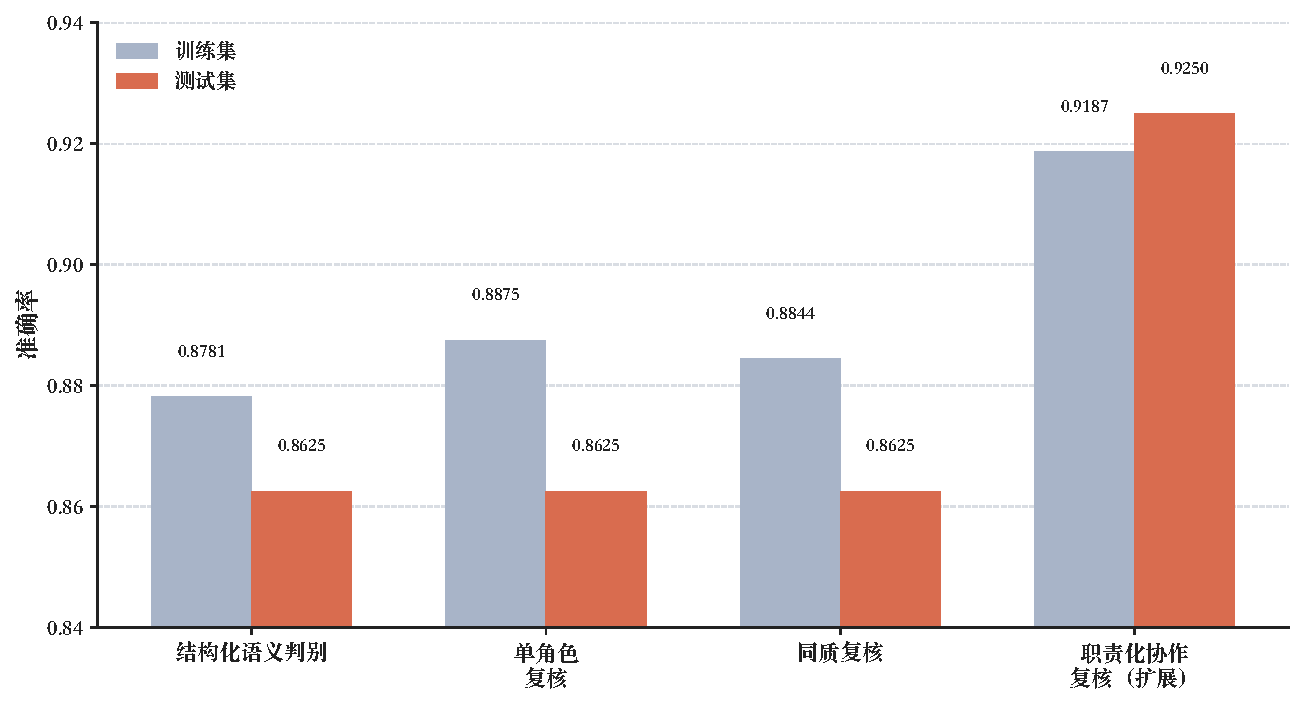
\includegraphics[width=0.88\linewidth]{figures/03_holdout3_collaboration_ablation.pdf}
\caption{扩展分布对齐子集上的协作复核协议比较。单角色复核与同质复核没有带来额外的 held-out \texttt{test} 收益，而职责化协作复核在 \texttt{expanded} 配置下显著提升了最终准确率。}
\label{fig:ablation}
\end{figure}

\subsection{收益出现在哪里：后验诊断分析}

为了分析修正主要出现在哪些类型的边界样本上，本文进一步报告若干后验诊断视角下的结果，如表~\ref{tab:main} 所示。

\begin{table}[H]
\centering
\caption{后验诊断分析结果。各行对应冻结 benchmark 上的不同诊断视角，而非独立 benchmark。}
\label{tab:main}
\resizebox{\linewidth}{!}{%
\begin{tabular}{lcccc}
\toprule
split & 规则路由 & 规则路由 + 协作复核 & 结构化语义判别 & 结构化语义判别 + 协作复核 \\
\midrule
常规揭盲样本 & 0.8286 & 0.8571 & 0.9143 & 0.9143 \\
困难边界样本 & 0.2917 & 0.4167 & 0.6250 & 0.6667 \\
fresh 样本 & 0.7407 & 0.7407 & 0.8889 & 0.9074 \\
\bottomrule
\end{tabular}
\vphantom{\rule{0pt}{1.1em}}%
}
\end{table}

后验诊断结果与主协议结论一致，并揭示了收益分布的主要来源。对于常规揭盲样本，结构化语义判别将准确率提升到 0.9143；对于困难边界样本，系统从 0.2917 提升到 0.6250，并在协作复核介入后达到 0.6667；对于 fresh 样本，系统从 0.7407 提升到 0.8889，并在协作复核介入后进一步达到 0.9074。主协议中的总体增益并非平均分布，而是更集中地出现在困难样本和 fresh 样本上。这一结果也解释了为什么协作复核不应被视为覆盖所有请求的统一慢路径，而更适合作为边界样本的条件化精修模块。

\subsection{执行负载代理}

由于 token 与 latency 日志尚未在所有 trace 中统一落盘，本文采用执行负载代理指标估计成本与修正效率。在代表性对比中，各协议的协作复核触发率与复核调用次数接近，而真正拉开差距的是 \texttt{Changed} 与 \texttt{Fixed} 数量。这说明当前方法的优势主要体现为在近似覆盖率下获得更高的净修正收益，决策质量而非调用规模构成了现阶段的主要区分因素。

\begin{figure}[tbp]
\centering
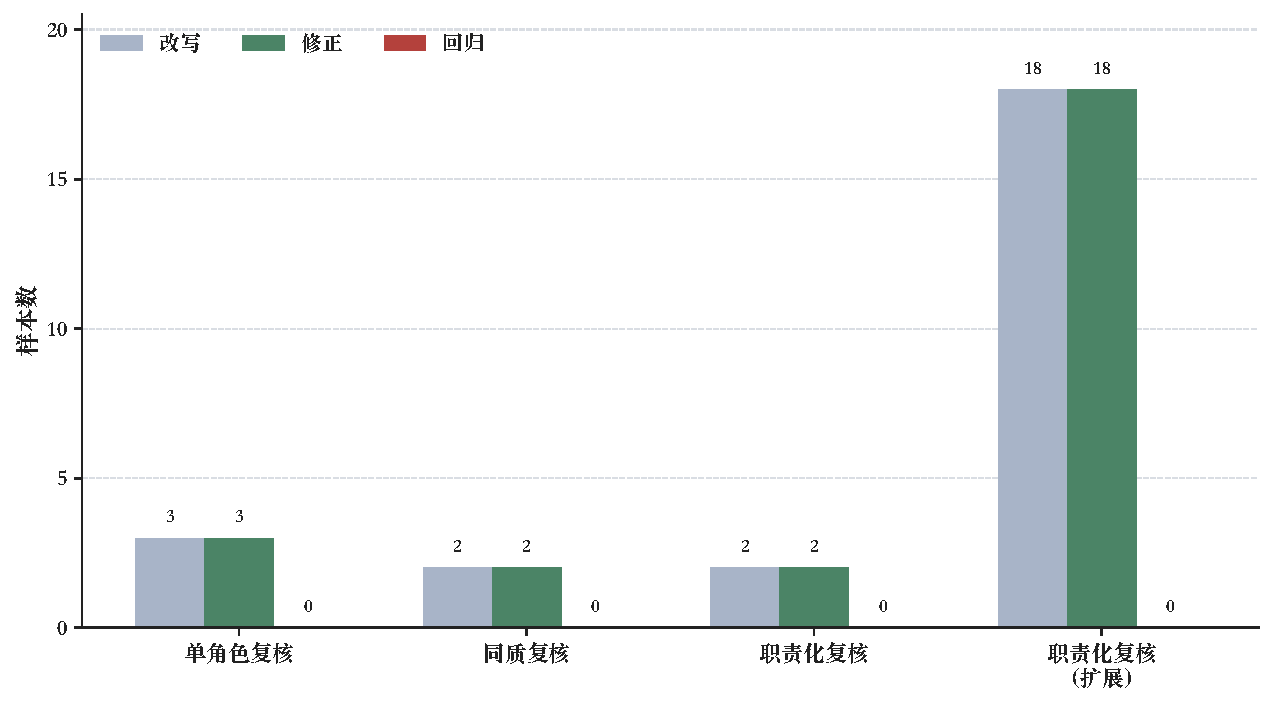
\includegraphics[width=0.86\linewidth]{figures/06_execution_proxy.pdf}
\caption{执行负载代理图。当前差异不在协作复核覆盖率，而在于相同覆盖率下的实际修正收益。}
\label{fig:proxy}
\end{figure}

\section{讨论}

本文的证据链支持一个比“协作越多越好”更窄、但也更稳的结论：在固定候选边界内，主要性能台阶来自结构化语义判别，而协作复核只有在职责化证据与决策配置对齐时才稳定产生净收益。

首先，统一 \texttt{train/test} 主协议下，规则路由到结构化语义判别的提升幅度显著大于默认协作复核的提升幅度。这说明本任务的首要瓶颈并不是“是否增加一次复核”，而是系统能否在候选集合内部显式表示竞争候选、混淆来源、粒度冲突和不确定性边界。只要这一步缺失，后续协作模块就很难获得足够细粒度的输入，从而只能在已有错误上重复判断。

其次，协作复核的收益并不自动成立。无论在统一主协议还是在扩展分布对齐子集上，最强结果都出现在 \texttt{expanded} 配置下，并且都表现为 \texttt{5 / 5 / 0} 的净修正；相反，单角色复核和同质复核并没有超过结构化语义判别基线。换言之，本文观察到的收益并不是“引入更多代理”本身带来的，而是角色异质性、语义交接质量和改判授权共同作用的结果。这一结论与近期关于多智能体讨论收益依赖控制协议和任务结构的研究观察一致\cite{bounds}，但本文把这一观察进一步落实到了固定候选边界内的受控改判问题上。

再次，协作复核的收益具有明显的样本结构。主文中的后验诊断显示，增益主要集中在困难边界样本、fresh 样本和扩展分布样本上，而在一部分常规样本上，直接路由已经足够稳定。这说明协作复核更适合作为复杂边界样本的条件化精修模块，而不是覆盖所有请求的统一慢路径。对语义路由系统而言，更有效的设计原则不是“普遍放大 deliberation”，而是把协作预算集中到最可能从职责化证据中获益的样本上。

最后，统一 trace 机制同样具有研究价值。由于系统显式记录候选快照、语义交接、角色提案和改判来源，错误分析可以从最终准确率回溯到具体阶段和具体样本。这不仅提高了结果的可解释性，也使本文的方法更接近可部署、可审计的决策系统，而不是一条不可追溯的黑箱推理链。

\section{局限性}

本文仍有三项主要限制。第一，当前结果建立在单一冻结 benchmark 上。尽管 held-out \texttt{test} 集未参与开发，但更大规模、更多来源、任务分布更广的独立验证仍然是检验结论外推性的必要步骤。第二，现有 trace 尚未在所有运行中统一落盘 token 与 latency，因此本文目前只能用执行负载代理刻画成本，而无法给出完整的质量--成本曲线。第三，执行落点解析模块已完成离线验证，但尚未在统一 runtime 中形成端到端联调结果，因此本文的主结论当前仍聚焦于语义路由本身，而不是完整执行链。

这些限制也对应了后续最直接的工作方向：补充独立验证集，统一质量--成本日志，并将当前冻结 lineage 整理为更系统的补充材料，使每一项结论都能够从原始 trace 精确回溯到最终表格与图示。

\section{结论}

本文研究了固定候选边界内的高可信语义路由，并把核心问题收敛为一个更具体的判断：协作复核在什么条件下才会稳定带来净收益。围绕 \texttt{563} 条样本的冻结 benchmark，实验结果表明，结构化语义判别建立了主要性能台阶，而协作复核只有在职责化证据与决策配置对齐时才持续带来修正收益。

因此，本文的核心结论不是“多代理讨论普遍有效”，而是对高可信语义路由而言，更有效的路径是固定候选边界内的结构化语义判别加受控协作改判。这个结论既解释了何时应该让协作模块介入，也为后续构建可部署、可审计的语义路由系统提供了更清晰的设计原则。

\appendix
\section{附录：实现细节与 Prompt Contract}
\label{appendix:prompt-contracts}

\subsection{评分细节与阈值模板}

为避免主文被实现层细节淹没，正文只保留定义方法身份的核心公式；更多打分模板、阈值和插值权重在附录中给出。

规则路由的 related 打分模板为
\begin{equation}
\label{eq:appendix-clean-related}
\begin{aligned}
r_{\mathrm{clean}}(c\mid x)=\;&
0.35\,\tilde s_R(c)
+0.18\,\phi_{\mathrm{sec}}(c)
+0.14\,\phi_{\mathrm{sup}}(c)\\
&+0.08\,\phi_{\mathrm{ctx}}(c)
+0.10\,\phi_{\mathrm{div}}(c)
+0.15\,\phi_{\mathrm{rel}}(c)
-\pi_{\mathrm{dup}}(c;\hat y_{\mathrm{clean}}).
\end{aligned}
\end{equation}

结构化语义判别的 related 融合模板为
\begin{equation}
\label{eq:appendix-semantic-related}
r_A(c\mid x)=
\beta_1 \widetilde r_{\mathrm{clean}}(c)
+ \beta_2 f_{\mathrm{rel}}(c)
+ \beta_3 f_{\mathrm{task}}(c)
+ b_{\mathrm{rel}}(c),
\end{equation}
其中 $\widetilde r_{\mathrm{clean}}$ 为规则 related 分数归一化结果，$f_{\mathrm{rel}}$ 对应候选级 \emph{related fit}，$b_{\mathrm{rel}}$ 奖励被显式挂为 related 的候选。

直接路由置信度模板为
\begin{equation}
\label{eq:appendix-semantic-confidence}
\mathrm{conf}_A(x)=
0.55\,p_A(\hat y_A\mid x)
+0.20\,\mathrm{margin}_A(x)
+0.15\,\mathrm{evidence}_A(x)
+0.10\,\mathrm{agree}_A(x),
\end{equation}
其中四项分别对应候选后验概率、top-1/top-2 间隔、显式证据支持度以及与规则路由的一致性。

若触发 round-2，协作复核的最终共识分数采用
\begin{equation}
\label{eq:appendix-final-consensus}
s_B(c\mid x)=
\begin{cases}
s_B^{(1)}(c\mid x), & \text{no round-2},\\
0.45\,s_B^{(1)}(c\mid x)+0.35\,s_B^{(2)}(c\mid x)+0.20\,s_A(c), & \text{otherwise}.
\end{cases}
\end{equation}

最终改判采用两阶段门控：先由 $g(x)$ 决定是否升级，再由最终改判门槛 $\tau_{\mathrm{rev}}$ 决定是否接受协作修正，即
\begin{equation}
\label{eq:appendix-final-decision}
(\hat y,\hat R)=
\begin{cases}
(\hat y_A,\hat R_A), & g(x)=0,\\
(\hat y_B,\hat R_B), & g(x)=1\ \text{and}\ \max_{c\in C_R(x)} M(c\mid x)\ge \tau_{\mathrm{rev}},\\
(\hat y_A,\hat R_A), & \text{otherwise}.
\end{cases}
\end{equation}

\subsection{诊断分析视角}

主文只报告统一 \texttt{train/test} benchmark 的核心结果，并将额外分析组织为后验诊断视角。具体而言，文中的“常规揭盲样本”“困难边界样本”“fresh 样本”和“扩展分布对齐子集”分别对应冻结 benchmark 上的若干标签化观察窗口，用于分析 fix 出现的样本类型、协作复核的收益分布以及不同决策配置在边界样本上的行为。它们服务于解释和消融，而不改变主 benchmark 的定义。

\subsection{直接路由的 Decision Packet}

结构化语义判别的 prompt 由固定 system prompt、固定 user rules 和动态 decision packet 组成。下面给出当前实现中使用的真实模板内容。

\paragraph{Stage A system prompt}
\begin{enumerate}[leftmargin=1.6em]
\item 你是 AgentDNS Stage A 的单智能体裁决器。
\item 你只能在给定候选集合内做结构化裁决，不能发明新 fqdn。
\item 请先理解 query 的 scene\_context、primary\_intent、secondary\_intents，再在 candidates 内判断 primary/related。
\item 你必须区分 primary 和 related；若不确定，应请求升级到 Stage B。
\item 除了裁决结果，请提供简短、受约束的语义摘要，说明为什么当前 primary 最合适、主要 challenger 为什么没有赢，以及你最不确定的点是什么。
\item confusion\_sources 只是软提示，不是既定事实。
\item 输出必须是单个 JSON 对象，不能附带散文解释。
\end{enumerate}

\paragraph{Stage A user rules}
\begin{enumerate}[leftmargin=1.6em]
\item \texttt{selected\_primary\_fqdn} 与 \texttt{selected\_related\_fqdns} 必须来自 \texttt{candidates}。
\item 先输出 \texttt{scene\_context}、\texttt{primary\_intent}、\texttt{secondary\_intents}。
\item 只有存在明确 \texttt{secondary\_intent} 且候选直接承接该意图时，related 才可填写。
\item 每个 \texttt{selected\_related\_fqdn} 都必须在 \texttt{candidate\_judgements.evidence\_for} 中给出具体短语支撑。
\item 在 governance/security 场景，不因“泛相关”默认挂 sibling 节点为 related。
\item \texttt{candidate\_judgements} 至少覆盖所有 candidates。
\item \texttt{task\_fit}、\texttt{primary\_fit}、\texttt{related\_fit} 取值范围均为 $[0,1]$。
\item \texttt{specificity\_judgement} 只能取 \texttt{too\_coarse / fit / too\_specific}。
\item \texttt{confidence} 取值范围为 $[0,1]$，但只作为模型自评。
\item 低置信、高风险或 primary/related 拿不准时，应设置 \texttt{escalate\_to\_stage\_b=true}。
\item 必须输出 \texttt{primary\_rationale}、\texttt{secondary\_rationale}、\texttt{uncertainty\_summary}。
\item \texttt{confusion\_points} 使用短标签列表，例如\\
\texttt{sibling\_granularity\_conflict}、\texttt{cross\_domain\_overlap} 等。
\item \texttt{override\_sensitivity} 只能取以下四类值：\\
\texttt{safe\_to\_override}、\texttt{needs\_strong\_evidence}、\\
\texttt{likely\_secondary\_confusion}、\texttt{high\_risk\_guarded}。
\item \texttt{challenger\_notes} 为对象列表，每项包含 \texttt{fqdn} 与 \texttt{note}。
\end{enumerate}

\paragraph{Stage A decision packet 字段}
\begin{enumerate}[leftmargin=1.6em]
\item 顶层字段：\texttt{sample\_id}、\texttt{namespace\_version}、\texttt{stage\_r\_version}、\\
\texttt{query}、\texttt{context}、\texttt{query\_view}、\texttt{hard\_rules}、\\
\texttt{soft\_hints}、\texttt{candidates}。
\item \texttt{query\_view} 包含：\texttt{full\_text}、\texttt{clauses}、\texttt{quoted\_segments}。
\item \texttt{soft\_hints} 包含：\texttt{confusion\_sources}、\texttt{selection\_signals}、\\
\texttt{top1\_candidate\_by\_stage\_r}、\texttt{top2\_candidate\_by\_stage\_r}、\\
\texttt{top1\_top2\_gap}。
\item 每个 candidate row 包含：\texttt{fqdn}、\texttt{score\_r}、\texttt{node\_kind}、\texttt{l1}、\texttt{l2}、\texttt{segment}、\\
\texttt{parent\_fqdn}、\texttt{fallback\_to}、\texttt{desc}、\texttt{aliases}、\texttt{source}、\\
\texttt{matched\_phrases}、\texttt{components}、\texttt{primary\_hits}、\\
\texttt{secondary\_hits}、\texttt{scene\_hits}。
\end{enumerate}

\paragraph{Stage A 输出字段}
\begin{enumerate}[leftmargin=1.6em]
\item 顶层输出：\texttt{scene\_context}、\texttt{primary\_intent}、\texttt{secondary\_intents}、\\
\texttt{selected\_primary\_fqdn}、\texttt{selected\_related\_fqdns}、\\
\texttt{candidate\_judgements}、\texttt{confidence}、\texttt{escalate\_to\_stage\_b}、\\
\texttt{escalation\_reasons}、\texttt{notes}。
\item 语义交接字段：\texttt{primary\_rationale}、\texttt{secondary\_rationale}、\\
\texttt{uncertainty\_summary}、\texttt{confusion\_points}、\\
\texttt{override\_sensitivity}、\texttt{challenger\_notes}。
\item 每个 \texttt{candidate\_judgement} 包含：\texttt{fqdn}、\texttt{task\_fit}、\\
\texttt{primary\_fit}、\texttt{related\_fit}、\texttt{specificity\_judgement}、\\
\texttt{risk\_mismatch}、\texttt{confidence}、\texttt{evidence\_for}、\\
\texttt{evidence\_against}。
\end{enumerate}

这些字段共同定义了从直接路由到协作复核的语义交接边界。尤其是 \texttt{uncertainty\_summary}、\texttt{confusion\_points} 和 \texttt{challenger\_notes}，直接决定了后续角色化复核看到的 handoff 信息。

\subsection{角色化复核 Packet}

协作复核同样由固定 system prompt、固定 user rules 和角色专属可见视图组成。

\paragraph{Stage B role system prompt 模板}
\begin{enumerate}[leftmargin=1.6em]
\item 你是 AgentDNS Stage B 的慢路径共识角色。
\item 你仍然只能在给定候选集合内输出最终提案，不能发明新 fqdn。
\item 你当前扮演的角色是某一职责家族。
\item 请结合 query、Stage A 的语义交接、以及候选内证据卡，比较 incumbent 与主要 challenger。
\item 如果视图里没有足够证据，请输出 neutral 或保守支持 Stage A 原判，而不是猜测。
\item 请说明 primary 为什么更像主任务，related 为什么更像次要诉求，以及你所负责维度上的最大歧义点。
\item 必须显式给出角色信号（support / block / neutral），不要替其他角色补做超出职责边界的判断。
\item 输出必须是单个 JSON 对象，不能附带散文解释。
\end{enumerate}

\paragraph{Stage B 角色专属 focus/rules}
\begin{enumerate}[leftmargin=1.6em]
\item \texttt{DomainExpert}：只负责 query 核心任务与候选能力是否直接匹配；必须给出 \texttt{task\_match} 维度上的 \texttt{support/block/neutral}。
\item \texttt{GovernanceRisk}：只负责治理、高风险、跨域边界是否允许 override；必须给出 \texttt{risk\_clearance} 维度上的 \texttt{support/block/neutral}。
\item \texttt{HierarchyResolver}：只负责 parent-child、base-segment、sibling competition 与粒度是否匹配；必须给出 \texttt{hierarchy\_judgement} 维度上的 \texttt{support/block/neutral}。
\item \texttt{UserPreference}：只负责主次意图、显式偏好和 related 线索；必须给出 \texttt{intent\_split} 维度上的 \texttt{support/block/neutral}。
\item \texttt{GeneralReviewer}：给出综合复核结论，用于非异质协作模式。
\end{enumerate}

\paragraph{Stage B user rules}
\begin{enumerate}[leftmargin=1.6em]
\item \texttt{proposal\_primary\_fqdn} 与 \texttt{proposal\_related\_fqdns} 必须来自 \texttt{candidates}。
\item \texttt{proposal\_primary\_fqdn} 必须唯一。
\item \texttt{proposal\_related\_fqdns} 可以为空，但不能包含 \texttt{proposal\_primary\_fqdn}。
\item \texttt{rationale} 需要解释为什么更支持当前 primary，以及 incumbent 与 challenger 的关键差异。
\item 若 \texttt{packet.round\_index=2}，应优先在 \texttt{round2\_candidates} 中比较。
\item \texttt{confidence} 取值范围为 $[0,1]$。
\item \texttt{override\_position} 只能是 \texttt{support\_stage\_a} 或 \texttt{propose\_override}。
\item 若 \texttt{override\_position=propose\_override}，\\
\texttt{override\_basis\_tags} 仅允许：\texttt{explicit\_primary\_evidence}、\\
\texttt{specificity\_gain}、\texttt{risk\_requirement}、\\
\texttt{multi\_intent\_separation}、\texttt{hierarchy\_disambiguation}。
\item 应优先利用当前 \texttt{role\_view} 中可见的证据，不假设被隐藏字段。
\item 若职责维度证据不足，应保守支持原判。
\item 对异质角色，额外输出：\texttt{role\_signal\_kind}、\\
\texttt{role\_signal\_polarity}、\texttt{role\_signal\_target\_fqdn}、\\
\texttt{role\_signal\_strength}、\texttt{role\_signal\_note}。
\end{enumerate}

\paragraph{角色可见视图}
\begin{enumerate}[leftmargin=1.6em]
\item 共享顶层字段：\texttt{sample\_id}、\texttt{namespace\_version}、\texttt{stage\_r\_version}、\\
\texttt{stage\_a\_version}、\texttt{stage\_b\_version}、\texttt{prompt\_version}、\\
\texttt{query}、\texttt{context}、\texttt{round\_index}、\texttt{stage\_a}、\\
\texttt{role\_scope}、\texttt{role\_view}、\texttt{candidates}，以及可选的 \texttt{round2\_candidates}。
\item \texttt{DomainExpert} 的可见 handoff：\texttt{scene\_context}、\texttt{primary\_intent}、\\
\texttt{primary\_rationale}、\texttt{override\_sensitivity}、\texttt{challenger\_notes}。\\
额外候选字段：\texttt{desc}、\texttt{aliases}、\texttt{positive\_evidence\_card}、\\
\texttt{negative\_evidence\_card}、\texttt{stage\_a\_llm\_task\_fit}、\\
\texttt{stage\_a\_llm\_primary\_fit}、\texttt{stage\_a\_llm\_evidence\_for}。
\item \texttt{GovernanceRisk} 的可见 handoff：\texttt{scene\_context}、\texttt{uncertainty\_summary}、\\
\texttt{confusion\_points}、\texttt{override\_sensitivity}。\\
额外候选字段：\texttt{negative\_evidence\_card}、\texttt{competition\_view}、\\
\texttt{stage\_a\_llm\_evidence\_against}。
\item \texttt{HierarchyResolver} 的可见 handoff：\texttt{primary\_intent}、\\
\texttt{uncertainty\_summary}、\texttt{confusion\_points}、\texttt{challenger\_notes}。\\
额外候选字段：\texttt{parent\_fqdn}、\texttt{matched\_phrases}、\\
\texttt{positive\_evidence\_card}、\texttt{negative\_evidence\_card}、\texttt{competition\_view}。
\item \texttt{UserPreference} 的可见 handoff：\texttt{scene\_context}、\texttt{primary\_intent}、\\
\texttt{secondary\_intents}、\texttt{secondary\_rationale}、\texttt{uncertainty\_summary}、\\
\texttt{confusion\_points}、\texttt{challenger\_notes}。\\
额外候选字段：\texttt{secondary\_recovery\_card}、\texttt{stage\_a\_llm\_related\_fit}、\\
\texttt{stage\_a\_llm\_specificity\_judgement}、\texttt{stage\_a\_llm\_evidence\_for}、\\
\texttt{stage\_a\_llm\_evidence\_against}。
\end{enumerate}

\paragraph{Stage B 输出字段}
\begin{enumerate}[leftmargin=1.6em]
\item 提案字段：\texttt{proposal\_primary\_fqdn}、\texttt{proposal\_related\_fqdns}、\\
\texttt{confidence}、\texttt{rationale}、\texttt{override\_position}、\texttt{override\_basis\_tags}。
\item 职责信号字段：\texttt{role\_signal\_kind}、\texttt{role\_signal\_polarity}、\\
\texttt{role\_signal\_target\_fqdn}、\texttt{role\_signal\_strength}、\texttt{role\_signal\_note}。
\end{enumerate}

这些字段共同支持正文中的 round-1/round-2 共识排序和责任式授权检查。

\subsection{为何将 Prompt 放入附录}

本文的主文只保留决定算法行为的三类对象：候选级分数、升级规则和改判授权规则。完整 prompt 文本、字段枚举和角色可见视图放在附录，是因为它们在功能上更接近可复现实验协议，而非需要在正文逐句展开的理论核心。对于当前任务，正文若直接插入长 prompt，会稀释方法主线；若完全省略结构化字段与角色视图，审稿人又无法判断系统是否真的可复现。因此，本稿采用“正文给公式与控制逻辑，附录给 packet 契约与 prompt 结构”的组织方式。

\begin{thebibliography}{99}

\bibitem{cot}
Wei, J., Wang, X., Schuurmans, D., et al.
\newblock Chain-of-Thought Prompting Elicits Reasoning in Large Language Models.
\newblock In \emph{NeurIPS}, 2022.

\bibitem{selfconsistency}
Wang, X., Wei, J., Schuurmans, D., et al.
\newblock Self-Consistency Improves Chain of Thought Reasoning in Language Models.
\newblock arXiv preprint arXiv:2203.11171, 2022.

\bibitem{tot}
Yao, S., Yu, D., Zhao, J., et al.
\newblock Tree of Thoughts: Deliberate Problem Solving with Large Language Models.
\newblock arXiv preprint arXiv:2305.10601, 2023.

\bibitem{debate}
Du, Y., Li, S., Torralba, A., Tenenbaum, J. B., Mordatch, I.
\newblock Improving Factuality and Reasoning in Language Models through Multiagent Debate.
\newblock arXiv preprint arXiv:2305.14325, 2023.

\bibitem{bounds}
Wang, Q., Wang, Z., Su, Y., Tong, H., Song, Y.
\newblock Rethinking the Bounds of LLM Reasoning: Are Multi-Agent Discussions the Key?
\newblock In \emph{ACL}, 2024.

\bibitem{routellm}
Ong, I., Almahairi, A., Wu, V., Chiang, W.-L., Wu, T., Gonzalez, J. E., Kadous, M. W., Stoica, I.
\newblock RouteLLM: Learning to Route LLMs with Preference Data.
\newblock arXiv preprint arXiv:2406.18665, 2024.

\bibitem{mixllm}
Wang, X., Liu, Y., Cheng, W., Zhao, X., Chen, Z., Yu, W., Fu, Y., Chen, H.
\newblock MixLLM: Dynamic Routing in Mixed Large Language Models.
\newblock In \emph{NAACL}, 2025.

\bibitem{cai}
Bai, Y., Kadavath, S., Kundu, S., et al.
\newblock Constitutional AI: Harmlessness from AI Feedback.
\newblock arXiv preprint arXiv:2212.08073, 2022.

\end{thebibliography}

\end{document}
